





\documentclass[
%  handout,
% serif,
% mathsans,
]
{beamer}
\usefonttheme[stillsansserifmath]{serif}
\usepackage[utf8]{inputenc}
% \usetheme[width=6ex]{Marburg}
% \usetheme[width=6ex]{Goettingen}
\usetheme[height=1cm]{Rochester}
\useinnertheme{circles}
% \useoutertheme[compress,subsection=false]{miniframes}
\usecolortheme{rose}
 \setbeamertemplate{navigation symbols}{}
\usepackage[T1]{fontenc}

\usepackage{csquotes}	



\usepackage{verbatim}
\usepackage{tikz}
\usetikzlibrary{shapes}                
\usetikzlibrary{fit}

% \renewcommand*\ttdefault{lmvtt}
% \renewcommand*\familydefault{\ttdefault} %% Only if the base font of the document is to be typewriter style


% \RequirePackage{emerald}
% \usepackage{comicsans}
% \usepackage{winfonts}

%\usepackage{pdfpages}
\usepackage{graphicx}

\usepackage{amsmath, amsthm}
% \usepackage{amssymb}
% \usepackage{ascii}
%  \usepackage{tikz}

 \RequirePackage{xcolor}
\RequirePackage[color,all,2cell]{xy}\SelectTips{cm}{12}\SilentMatrices\UseAllTwocells  % commutative diagrams

\usepackage{bussproofs}

\definecolor{dkblue}{rgb}{0,0.1,0.5}
\definecolor{lightblue}{rgb}{0,0.5,0.5}
\definecolor{dkgreen}{rgb}{0,0.4,0}
\definecolor{dk2green}{rgb}{0.4,0,0}
\definecolor{dkviolet}{rgb}{0.6,0,0.8}

% \usepackage{arev}
\usepackage{listings}
\newcommand{\sss}{\ttfamily\bfseries\small}
\def\lstlanguagefiles{defManSSR.tex}\lstset{language=SSR}

% \usepackage[bitstream-charter]{mathdesign}
%  \usepackage{palatino}\linespread{1.05}
% \usepackage{verbatim}

\title[Comodules over relative comonads]{Comodules over relative comonads \\ for streams and infinite matrices}
\author[B.\ Ahrens and R.\ Spadotti]{Benedikt Ahrens \\~\\ joint work with R\'egis Spadotti}
% \date{2011--09--11}
% \date{Sept 11, 2011}
\date[2014-04-05/06]{CMCS 2014}
%{19th Workshop on \\ Logic, Language,  Information and Computation}

\institute[IRIT] % (optional, but mostly needed)
{%
%   Centre International de Math\'ematique et Informatique de Toulouse\\
  Institut de Recherche en Informatique de Toulouse\\
   Universit\'e Paul Sabatier\\ ~ \\
%     \includegraphics[height=1em]{logo_irit.jpg} 
%          \hspace{1cm} \includegraphics[height=1em]{logo_ups.jpg}
%   Equipe ACADIE
}

\setbeamertemplate{footline}
{%
  \leavevmode%
  \hbox{\begin{beamercolorbox}[wd=.5\paperwidth,ht=2.5ex,dp=1.125ex,leftskip=.3cm plus1fill,rightskip=.3cm]{author in head/foot}%
    \usebeamerfont{author in head/foot}\insertshortauthor
  \end{beamercolorbox}%
  \begin{beamercolorbox}[wd=.5\paperwidth,ht=2.5ex,dp=1.125ex,leftskip=.3cm,rightskip=.3cm plus1fil]{title in head/foot}%
    \usebeamerfont{title in head/foot}\insertshorttitle\hfill\insertframenumber/\inserttotalframenumber
  \end{beamercolorbox}}%
  \vskip0pt%
}

\newcommand{\constfont}[1]{\ensuremath{\mathsf{#1}}}

\newcommand{\C}{\mathcal{C}}
\newcommand{\D}{\mathcal{D}}
\newcommand{\N}{\mathbb{N}}
\newcommand{\bind}[2]{{#1}\mathbin{\gg\hspace{-.8ex}=}{#2}}
\newcommand{\Tri}{\constfont{Tri}}
\newcommand{\stream}{\constfont{Stream}}
\newcommand{\head}{\constfont{top}}
\newcommand{\tail}{\constfont{rest}}
\newcommand{\shead}{\constfont{head}}
\newcommand{\stail}{\constfont{tail}}
\newcommand{\cosubst}{\constfont{cosubst}}
\newcommand{\bisim}{\constfont{bisim}}
\newcommand{\redec}{\constfont{redec}}
\newcommand{\cut}{\constfont{cut}}
\newcommand{\ccut}{\constfont{ccut}}
\newcommand{\RComonad}{\constfont{RComonad}}
\newcommand{\RComonadWC}{\constfont{\RComonad wCut}}
\newcommand{\ULCop}{\constfont{LC}}
\newcommand{\induced}[1]{\ensuremath{\langle {#1} \rangle}}

\newcommand{\comp}[2]{\ensuremath{{#2} \circ {#1}}}

\newcommand{\shift}{\constfont{shift}}
\newcommand{\lift}{\constfont{lift}}
\newcommand{\abs}{\constfont{abs}}
\newcommand{\subst}{\constfont{subst}}
\newcommand{\Setoid}{\constfont{Setoid}}
\newcommand{\eq}{\ensuremath{\mathsf{eq}}}
\newcommand{\App}{\constfont{App}}
\newcommand{\Abs}{\constfont{Abs}}
\newcommand{\Var}{\constfont{Var}}
\newcommand{\var}{\constfont{var}}
\newcommand{\unit}{\constfont{unit}}
\newcommand{\coq}{\texttt{Coq}\xspace}
\newcommand{\monbind}{\constfont{bind}}

%  \newcommand{\bind}[2]{{#1} \blacktriangleright {#2}}
% \newcommand{\bind}[2]{{#1} \mathbin{\vartriangleright} {#2}}
% \newcommand{\bind}[2]{{#1} \mathbin{\mathbf{\rhd}} {#2}}
\newcommand{\LC}{\mathsf{LC}}
\newcommand{\TLC}{\mathsf{TLC}}
\newcommand{\PCF}{\mathsf{PCF}}

\newcommand{\Id}{\mathsf{Id}}


\newcommand{\Set}{\constfont{Type}}
\newcommand{\PreOrd}{\mathsf{Pre}}

\newcommand{\PCFar}{\Rightarrow}
\newcommand{\Bool}{Bool}
\newcommand{\Nat}{Nat}

\DeclareMathOperator{\dom}{dom}
\DeclareMathOperator{\cod}{cod}

\newcommand{\init}[1]{\hat{#1}}
\newcommand{\retyping}[1]{\vec{#1}}

\newcommand{\fat}[1]{\textbf{#1}}

\AtBeginSection[]
 {
    \begin{frame}
        \frametitle{Outline}
        \tableofcontents[currentsection]
    \end{frame}
 }


\begin{document}

\begin{frame}
 \titlepage
\end{frame}


\begin{frame}
 \frametitle{Goal}
 
   \begin{itemize}\setlength{\itemsep}{1em}
    \item Category-theoretic semantics of \fat{co}inductive data types
          in intensional Martin-L\"of type theory
    \item [$\leadsto$] Develop a notion of \enquote{coalgebra} for the signature of a codata type
    \item Incorporate canonical cosubstitution
   \end{itemize}

%   \begin{block}{In this talk we consider}
%    \begin{itemize}
%     \item []  the codata type of \fat{infinite triangular matrices}
%    \end{itemize}
%   \end{block}

%   TODO: make goal slide
 
\end{frame}


\begin{frame}
 \frametitle{Outline}
 \tableofcontents
\end{frame}


\section{Syntax: inductives and substitution}

\begin{comment}
\begin{frame}
 \frametitle{Starting point: W-types in Martin-L\"of TT}
 
  
 \begin{block}{Well-founded trees as \fat{initial algebra} of polynomial functor}
 
  \begin{itemize}
   \item Trees specified by $A$ and $x:A\vdash B(x)$
   
   \item Type of natural numbers $\mathbb{N} := W~A~B$ with: \[A = \{O,S\}, \quad B(O) = \{\}, \quad B(S)=\{*\}\]
 
   \item The type $W~A~B$ is the (carrier of) the initial algebra of
    \[X \mapsto \sum_{a:A}X^{B(a)} \]
 
 
   
   \item Dybjer '97, Moerdijk and Palmgren '00
  \end{itemize}
 \end{block}
\end{frame}
\end{comment}

\begin{frame}
  \frametitle{Heterogeneous data types}

%  \begin{block}{Initial semantics extended to some \fat{heterogeneous} inductives}
 
  \begin{description}
    \item [Motivation:] \fat{binding syntax} 
%               modelled through %($\lambda$-calculus)    \fat{heterogeneous} data type
           \begin{align*} \LC(X : \Set) \enspace ::=                                              
                                           \enspace  & \Var : X \to \LC(X) \\
                                           | \enspace  & \App : \LC(X)\times\LC(X)\to\LC(X) \\ 
                                           | \enspace &\Abs : \LC(X + 1) \to \LC(X) \enspace
           \end{align*}
    \item [Heterogeneity of $\Abs$:] \hfill \\ recursive argument with bigger parameter $X+1$
    
    \item [Substitution:] \hfill\\        
       $ \subst_{X,Y} : \bigl(X \to \LC (Y)\bigr) \to \LC (X) \to \LC (Y) $
    
    \item [Avoiding capture:] \hfill \\ $\shift_{X,Y} : \bigl(X \to \LC(Y)\bigr) \to X+1 \to \LC(Y+1)$
    
%    \begin{itemize}
%     \item 
  \end{description}
%     \item variant using monads: Altenkirch \& Reus '99, Hirschowitz \& Maggesi '07, '10
%    \end{itemize}
%  \end{block} 
\end{frame}

\begin{frame}
 \frametitle{Initial semantics for binding syntax}
    
    \begin{block}{Initial semantics for lambda calculus: Fiore, Plotkin \& Turi '99}
      \begin{itemize}
       \item characterizes not only data type but also \fat{substitution} %operation
       \item reformulated using \fat{monads} by Hirschowitz \& Maggesi '07
      \end{itemize}
    \end{block}

  Basis for this reformulation:
    
    \begin{lemma}[Substitution is monadic: Altenkirch \& Reus '99]
       \begin{itemize}
         \item [] $(\LC, \Var, \subst)$ forms a monad (in Kleisli form)
       \end{itemize}

    \end{lemma}

    
%     
%     \begin{block}{Reformulation by H \& M}
%        \begin{itemize}
%            \item uses Altenkirch \& Reus '99 \\ lambda calculus \fat{+ substitution} forms a \fat{monad}
%            \item Lambda calculus as \fat{initial} monad 
%               \begin{itemize}
%                  \item [$\leadsto$]actually: monad + \enquote{algebra} structure for constructors
%               \end{itemize}
%            \item notion of \fat{module over a monad} 
%                \begin{itemize}
%                  \item [$\leadsto$]used to characterize constructors of lambda calculus
%                \end{itemize}
%        \end{itemize}
%     \end{block}

\end{frame}

\begin{frame}
 \frametitle{Initial semantics for $\lambda$-calculus using monads}
   \begin{definition}[Algebra for signature of $\LC$, H \& M '07]
     \begin{itemize}
      \item a monad $(T, \unit, \monbind)$ on $\Set$
      \item two \fat{morphisms of modules over $T$},
         \vspace{-.5em}
          \begin{align*}
               App &: T \times T \to T \\
               Abs &: T(\_ + 1) \to T   
          \end{align*}
          
         \vspace{-1.5em}
         
     \end{itemize}

   \end{definition}
   
   
   \pause
   
   \enquote{Module morphism} expresses \fat{commutativity with $\monbind$}:
   \begin{align*} \comp{App}{\monbind~f} \quad &= \quad \comp{(\monbind~f)^2}{App}  \\
                  \comp{Abs}{\monbind~f} \quad &= \quad \comp{\monbind~(\shift~f)}{Abs}
      \end{align*}
   \vspace{-1em}
   
   \pause 
   
   \begin{lemma}[Initial semantics for $\LC$, H \& M '07]
      $(\LC, \App, \Abs)$ is the initial algebra, where $\LC = (\LC,\Var,\subst)$
   \end{lemma}


\end{frame}



\begin{frame}
 \frametitle{Goal: characterize \fat{co}data types with \fat{co}substitution}
 
\begin{block}{Goal}
dualize techniques of H \& M to characterize
  \begin{itemize}
    \item
         \fat{co}data types in \fat{intensional ML type theory} with 
    \item\fat{co}substitution 
  \end{itemize}
    as  \fat{terminal} object
%     \item I.e.: Given a heterogeneous codata type, what is the category in which that codata type is terminal?
  
 \end{block}
  
\begin{block}{In this talk}
 
  \begin{itemize} 
    \item  streams
    \item  infinite triangular matrices
  \end{itemize}
  
\end{block} 
\end{frame}


\begin{comment}
\begin{frame}
 \frametitle{Binding signatures with (in)equations}
   \begin{block}{Equational theories}
    \begin{itemize}
     \item prime example: lambda calculus modulo $\beta$-equivalence
     \item Fiore with students Hur \& Mahmoud
     \item Hirschowitz \& Maggesi 
    \end{itemize}
   \end{block}
   
  \begin{block}{Reduction rules via \fat{in}equations}
   \begin{itemize}
    \item A., PhD thesis: 
     \begin{itemize}
      \item based on ideas by Hirschowitz \& Maggesi
      \item uses notion of \fat{relative} monad (Altenkirch et al. '10)
     \end{itemize}
   \end{itemize}
  \end{block}
  
  \begin{block}{Goal:}
   do the same for cosyntax, i.e.\ \fat{nested co}data types 
  \end{block}
\end{frame}
\end{comment}

\section{Homogeneous cosyntax: streams}


\begin{frame}
 \frametitle{Streams over a base type}
 
 \begin{itemize}
   \item Streams = infinite lists over some base type $A$
 
  \begin{center}
  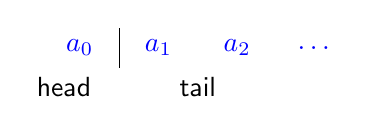
\begin{tikzpicture}
      \foreach \x in {0,...,2}{\draw (\x,0) node[color=blue]{$a_{\x}$};};
      \draw (3,0) node[color=blue]{$\dots$};
      \draw (0.5,0.25)--(0.5,-0.25);
      \draw (-0.2,-0.5) node{$\shead$};
      \draw (1.5,-0.5) node{$\stail$};
  \end{tikzpicture}
                                       
 \end{center}
 
 \item Specified by destructors
 
 \begin{center}
 
  \def\proofSkipAmount{\vskip.8ex plus.8ex minus.4ex}
    \AxiomC{$s : \stream(A)$}\doubleLine
     \UnaryInfC{$\shead_A(s) : A$}
      \DisplayProof
      \hspace{3em}
%                       
%  
%  \vspace{15ex}
%  
  \AxiomC{$s : \stream(A)$}\doubleLine
                                       \UnaryInfC{$\stail_A(s) : \stream(A)$}
                                       \DisplayProof%

 \end{center}
 
   \vspace{2ex}

 \item \enquote{Sameness} = bisimilarity in IMLTT
  \begin{center}
                                            \def\extraVskip{3pt}
     \def\proofSkipAmount{\vskip.8ex plus.8ex minus.4ex}
    \AxiomC{$s \sim s'$}\doubleLine
     \UnaryInfC{$\shead(s) = \shead(s')$}
      \DisplayProof
                        \hspace{3em}
                                       \AxiomC{$s \sim s'$}\doubleLine
                                       \UnaryInfC{$ \stail(s) \sim \stail(s')$}
                                       \DisplayProof   
  \end{center}
  \end{itemize}
\end{frame}

\begin{frame}
 \frametitle{Structure on streams}
  
  \begin{itemize}\setlength{\itemsep}{1em}
   \item $(\stream A, \sim)$ is a \emph{setoid}, \[\stream : \Set \to \Setoid\]
   \item Canonical cosubstitution
          \[ \cosubst: (\stream A \to B) \to \stream A \to \stream B \]
         is compatible with bisimilarity:
          \[ \cosubst: \Setoid(\stream A , \eq B) \to \Setoid(\stream A , \stream B) \]
         with
         \[ \eq : \Set \to \Setoid  \qquad \eq \dashv \constfont{forget}\]         
  \end{itemize}
\end{frame}

\begin{frame}
 \frametitle{Structure on streams}
 
 \begin{lemma}
  $(\stream,\shead,\cosubst)$ is a \fat{comonad relative to $\eq:\Set\to\Setoid$}.
 \end{lemma}

 \begin{definition}[\fat{Relative} (co)monad, Alten., Chapm. \& Uust.\ '10]
  \begin{itemize} 
   \item underlying functor is \fat{not} necessarily \fat{endo}
   \item needs \enquote{mediating} functor (above: $\eq$)
  \end{itemize}
\end{definition}
\end{frame}

\begin{frame}
 \frametitle{About the destructor $\stail$}
 
 \begin{block}{Morphisms of modules over monads}
%   \begin{itemize}
%    \item used in work by Hirschowitz and Maggesi
%    \item 
   characterize distributivity of substitution over constructors
%       \begin{align*} \bind{\App~(s,t)}{f} \quad &= \quad \App~(\bind{s}{f},\bind{t}{f}) \\
%                      \bind{\Abs~t}{f}       \quad &= \quad \Abs~(\bind{t}{\shift~f}) 
%       \end{align*}
%   \end{itemize}

         \[ \App : \LC\times\LC \to \LC \]
%          \[ \subst~f~(\App~s~t) = \App~(\subst~f~s)(\subst~f~t) \]
         \[ \comp{\App}{\subst~f} = \comp{(\subst~f)^2}{\App} \]

 \end{block}

 \begin{block}{Morphisms of \fat{co}modules over \fat{relative co}monads}
%   \begin{itemize}
%    \item 
   characterize distributivity of \fat{co}substitution over destructors
%    \item %example of morphism of comodules:  
         \[\stail : \stream \to \stream\]
%              \[\stail~(\cosubst~f~t) = \cosubst~f~(\stail~t) \]
          \[ \comp{\cosubst~f}{\stail} = \comp{\stail}{\cosubst~f} \]
%   \end{itemize}
 \end{block} 
 
\end{frame}


\begin{frame}
 \frametitle{Terminal semantics for $\stream$}
 
  \begin{definition}[Category of coalgebras]
    A coalgebra for the signature of $\stream$ is given by a pair $(S,t)$:
    \begin{itemize}
     \item a comonad $S$ relative to $\eq: \Set \to \Setoid$
     \item a morphism of comodules over $S$
        \[  t : S \to S \]
    \end{itemize}
   Morphisms: \ldots
  \end{definition}

 \begin{lemma}
  $(\stream,\stail)$ is the terminal object in the above category.
 \end{lemma}
  
\end{frame}


\section{Heterogeneous cosyntax: infinite triangular matrices}

\begin{frame}
 \frametitle{An example of cosyntax: infinite triangular matrices}
 
   \begin{block}{\Tri: the codata type of infinite triangular matrices}
     \begin{itemize}
      \item omit redundant information below the diagonal
      \item have a \fat{variable} type $A$ of diagonal elements 
        \begin{itemize} 
          \item e.g.\ invertible elements
        \end{itemize}
      \item a fixed type $E$ of elements for rest of matrix
      \item usage: Pascal matrices (binomial coefficients), mathematical physics (infinite-dim.\ problems)
     \end{itemize}
   \end{block}
   
   
\begin{center}
   
 
%
  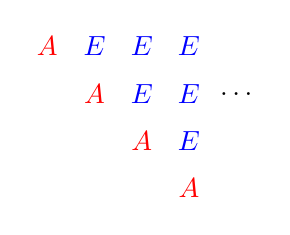
\begin{tikzpicture}[scale = 0.6]
     \foreach \y in {0,...,2}
     {\foreach \x in {\y,...,2}
       \draw (\x+1, -\y) node[color=blue]{$E$} ;
     }
     \foreach \x in {0,...,3} \draw (\x, -\x) node[color=red]{$A$} ;
     \draw(4,-1) node{$\ldots$};
%      \draw[style = dashed](0.5,0.2) -- (0.5,-1.2);
%      \draw[style = dashed](1.5,0.2) -- (1.5,-2.2);
%      \draw[style = dashed, thin](2.5,0.2) -- (2.5,-3.2);
     
%      \draw[color=green]  (3,0.5) -- (0.3,0.5) -- (0.3,
%      -1.2)  -- (2.8,-3.6);
%      \draw[color=green, dashed]  (3,0.5) -- (4,0.5);
%      \draw[color=green, dashed]  (2.8,-3.6) -- (3.5,-4.2);
 \end{tikzpicture}

\end{center}
 

   
\end{frame}

\begin{frame}
 \frametitle{Matrices through trapezia: the destructors of $\Tri$}
 
 
 
\begin{columns}

 \column{.4\textwidth}
 
 \begin{center}
 
  \def\proofSkipAmount{\vskip.8ex plus.8ex minus.4ex}
    \AxiomC{$t : \Tri(A)$}\doubleLine
     \UnaryInfC{$\head_A(t) : A$}
      \DisplayProof
                      
 
 \vspace{15ex}
 
  \AxiomC{$t : \Tri(A)$}\doubleLine
                                       \UnaryInfC{$\tail_A(t) : \Tri(E\times A)$}
                                       \DisplayProof%
 
 \end{center}
 
 \vspace{5ex}
 
 \column{.5\textwidth}

\vspace{2em}
 
  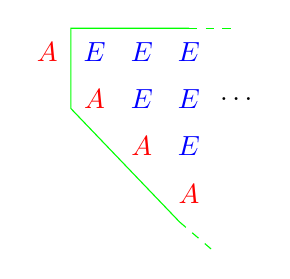
\begin{tikzpicture}[scale = 0.6]
     \foreach \y in {0,...,2}
     {\foreach \x in {\y,...,2}
       \draw (\x+1, -\y) node[color=blue]{$E$} ;
     }
     \foreach \x in {0,...,3} \draw (\x, -\x) node[color=red]{$A$} ;
     \draw(4,-1) node{$\ldots$};
%      \draw[style = dashed](0.5,0.2) -- (0.5,-1.2);
%      \draw[style = dashed](1.5,0.2) -- (1.5,-2.2);
%      \draw[style = dashed, thin](2.5,0.2) -- (2.5,-3.2);
     
     \draw[color=green]  (3,0.5) -- (0.5,0.5) -- (0.5,
     -1.2)  -- (2.8,-3.6);
     \draw[color=green, dashed]  (3,0.5) -- (4,0.5);
     \draw[color=green, dashed]  (2.8,-3.6) -- (3.5,-4.2);
 \end{tikzpicture}
 
\vspace{5ex}
 
  \begin{overprint}
    \onslide<2>
\hspace{1em}    
	  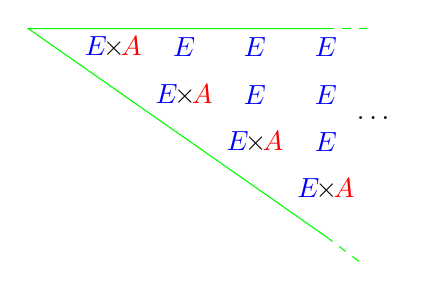
\begin{tikzpicture}[scale = 0.6]
	  \foreach \y in {0,...,2}
	    {\foreach \x in {\y,...,2}
	      \draw (1.5*\x+10.5, -\y) node[color=blue]{$E$} ;
	    }
	    \foreach \x in {0,...,3} \draw (1.5*\x+9, -\x)
	    node{{\color{blue}\textbf{$E$}} \hspace*{-.8em} $\times$ \hspace*{-.8em} {\color{red} $A$}} ;
	    \draw(14.5,-1.5) node{$\ldots$};
	    
	    \draw[color=green] (13.5,0.4) -- (7.2,0.4) -- (13.5, -4); 
	    \draw[color=green, dashed] (13.5,0.4) -- (14.4,0.4) ; 
	    \draw[color=green, dashed] (13.5,-4) -- (14.3,-4.6) ; 
	  \end{tikzpicture}
    \onslide<1>
\hspace{1em}
	    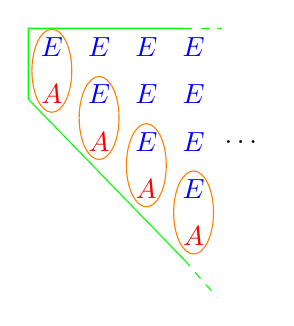
\begin{tikzpicture}[scale = 0.6]
	    % matrix coefficients
	    \foreach \y in {0,...,2}
	    {\foreach \x in {\y,...,2}
	      \draw (\x+1, -\y) node[color=blue]{$E$} ;
	    }
	    \foreach \x in {0,...,3} \draw (\x, -\x-1) node[color=red]{$A$} ;
	    \foreach \x in {0,...,3} \draw (\x, -\x)
	    node[color=blue]{\textbf{$E$}} ;
	    \draw(4,-2) node{$\ldots$};
	    
	    % green border
	    \draw[color=green] (2.8,0.4) -- (-0.5,0.4) -- (-0.5, -1.1) --
	    (2.8,-4.5)  ; 
	    \draw[color=green, dashed] (2.8,0.4) -- (3.6,0.4) ; 
	    \draw[color=green, dashed] (2.8,-4.5) -- (3.5,-5.3) ; 
	    
	    % ellipses around pairs of A and E
	    \draw[color=orange](0, -0.5) ellipse (12pt and 25pt) ;  
	    \draw[color=orange](1, -1.5) ellipse (12pt and 25pt) ;  
	    \draw[color=orange](2, -2.5) ellipse (12pt and 25pt) ;  
	    \draw[color=orange](3, -3.5) ellipse (12pt and 25pt) ;  
	  \end{tikzpicture}
  \end{overprint}
 
 
  \end{columns}
\end{frame}  


  
 

\begin{frame}
 \frametitle{Redecoration}
 
 
 \[\redec_{A,B} : (\Tri A \to B) \to (\Tri A \to \Tri B) \]
 \begin{center}
 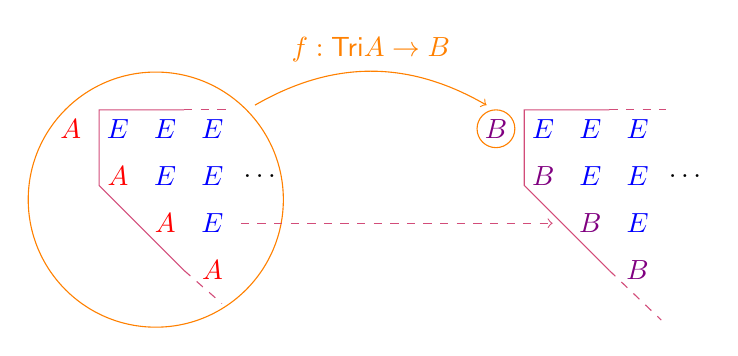
\begin{tikzpicture}[scale = 0.6]
    \foreach \y in {0,...,2}
    {\foreach \x in {\y,...,2}
      \draw (\x+1, -\y) node[color=blue]{$E$} ;
    }
    \foreach \x in {0,...,3} \draw (\x, -\x) node[color=red]{$A$} ;
    \draw(4,-1) node{$\ldots$};

    \foreach \y in {0,...,2}
    {\foreach \x in {\y,...,2}
      \draw (\x+10, -\y) node[color=blue]{$E$} ;
    }
    \foreach \x in {0,...,3} \draw (\x+9, -\x) node[color=violet]{$B$} ;
    \draw(13,-1) node{$\ldots$};
    \draw[color=purple!70]  (2.4, -3) --
    (0.6,-1.2) -- (0.6,0.4) -- (2.4,0.4);
    \draw[color=purple!70, dashed]  (2.4,0.4) -- (3.4,0.4);
    \draw[color=purple!70, dashed]  (2.4,-3) -- (3.2,-3.7);
 
    \draw[color=orange] (1.8,-1.5) circle(2.7cm);

    \draw[color=purple!70]  (11.4, -3) --
    (9.6,-1.2) -- (9.6,0.4) -- (11.4,0.4);
    \draw[color=purple!70, dashed]  (11.4,0.4) -- (12.6,0.4);
    \draw[color=purple!70, dashed]  (11.4,-3) -- (12.5,-4.05);
    
    \draw[color=orange] (9,0) circle(0.4cm);
    
    \draw[->,color = orange] (3.9,0.5) to [bend left] node[auto,
    swap, above]{$f:\Tri A \to B$} (8.8,0.5) ; 

    \draw[->,color = purple!70, dashed] (3.6,-2) to (10.2,-2) ; 
  \end{tikzpicture}
 \end{center}
 
%  When redecorating the $\tail$ of the matrix, we need a function \[\lift~f : \Tri(E\times A) \to E \times B\]
%   \[ \tail (\redec~f~t) \quad = \redec~(\lift~f) (\tail~t) \]
  
  \vspace{-6ex}
  
%    \begin{align*}\head\bigl(\redec~f~t\bigr) &:= f~t \quad\text{ and } \\
%                      \tail\bigl(\redec~f~t\bigr) &:= \redec\bigl(\lift~f\bigr)(\tail~t) \enspace .
%    \end{align*}
  \begin{align*} \comp{\redec~f}{\head} &:= f \quad\text{ and } \\
                 \comp{\redec~f}{\tail} &:= \comp{\tail}{\redec~(\lift~f)} \enspace .
   \end{align*}
  
  with $\quad\lift~f : \Tri(E\times A) \to E \times B$
   
\end{frame}

\begin{frame}
 \frametitle{$\Tri$ is a weak constructive comonad}
  \begin{block}{Sameness = \fat{bisimilarity}}
    Bisimilarity $\sim$ coinductively defined via destructors
     
    \begin{center}
                                            \def\extraVskip{3pt}
     \def\proofSkipAmount{\vskip.8ex plus.8ex minus.4ex}
    \AxiomC{$t \sim t'$}\doubleLine
     \UnaryInfC{$\head(t) = \head(t')$}
      \DisplayProof
                        \hspace{3ex}
                                       \AxiomC{$t \sim t'$}\doubleLine
                                       \UnaryInfC{$ \tail(t) \sim \tail(t')$}
                                       \DisplayProof   
   \end{center}                                    
  \end{block}
  
  \begin{lemma}[Matthes and Picard '11]
      $(\Tri : \Set \to \Set, \head, \redec)$ forms a \enquote{weak constructive comonad}.
  \end{lemma}
  
  \begin{itemize}
   \item [$\leadsto$] \enquote{weak constructive} refers to compatibility conditions with bisimilarity
  \end{itemize}

\end{frame}
   
\begin{frame}
 \frametitle{$\Tri$ is a relative comonad}
  \begin{block}{Alternatively, $\Tri A$ is a \fat{setoid} rather than a (plain) type}
%     \begin{itemize}
       \vspace{-2em}
           \begin{align*} 
                 \head_A &: \Setoid(\Tri A, \eq A) \\
                 \redec_{A,B} &: \Setoid(\Tri A,\eq B) \to \Setoid(\Tri A,\Tri B )
           \end{align*}
       
%        \vspace{-1em}
       
             with $\eq : \Set \to \Setoid$
%     \end{itemize}

  \end{block}

\pause
  \begin{lemma}[Reformulation of Matthes and Picard '11]
 $(\Tri : \Set\to\Setoid, \head, \redec)$ forms a \fat{comonad relative to} $\eq:\Set\to\Setoid$.
\end{lemma}




\end{frame}


% \section{Coinitiality for $\Tri$}

\begin{comment}
\begin{frame}
 \frametitle{Towards \enquote{coalgebras} for the signature of $\Tri$}
 
  \begin{block}{Goal: define \enquote{coalgebra} s.t.\ $\Tri$ is (the terminal) one}
    More specifically:
    \begin{itemize}
     \item define a notion of \enquote{morphism} for destructor $\tail$
     \item requirement: want to capture interplay of $\tail$ and $\redec$:
       \[\tail\bigl(\redec~f~t\bigr) = \redec\bigl(\lift~f\bigr)(\tail~t)\]
    \end{itemize}
  \end{block}

 \begin{block}{Analogous situation for syntax:}
   For the lambda calculus with monadic substitution:
      \[ \subst~f~(\Abs~t) = \Abs~(\subst~(\shift~f)~t) \]
 \end{block}
\end{frame}
\end{comment}


\begin{frame}
 \frametitle{(Co)modules over (relative) (co)monads}
 \begin{block}{Morphisms of modules over monads}
%   \begin{itemize}
%    \item used in work by Hirschowitz and Maggesi
%    \item 
   characterize distributivity of substitution over constructors
%       \begin{align*} \bind{\App~(s,t)}{f} \quad &= \quad \App~(\bind{s}{f},\bind{t}{f}) \\
%                      \bind{\Abs~t}{f}       \quad &= \quad \Abs~(\bind{t}{\shift~f}) 
%       \end{align*}
%   \end{itemize}

         \[ \Abs : \LC(\_ + 1) \to \LC \]
%          \[ \subst~f~(\Abs~t) = \Abs~(\subst~(\shift~f)~t) \]
         \[ \comp{\Abs}{\subst~f} = \comp{\subst~(\shift~f)}{\Abs} \]
 \end{block}

 \begin{block}{Morphisms of \fat{co}modules over \fat{relative co}monads}
%   \begin{itemize}
%    \item 
   characterize distributivity of \fat{co}substitution over destructors
%    \item %example of morphism of comodules:  
         \[\tail : \Tri \to \Tri(E\times \_)\]
%              \[\tail~(\redec~f~t) = \redec~(\lift~f)~(\tail~t) \]
         \[\comp{\redec~f}{\tail} = \comp{\tail}{\redec~(\lift~f)} \]
%   \end{itemize}
 \end{block} 
\end{frame}

\begin{frame}
 \frametitle{Coalgebras for the signature of $\Tri$}
  \begin{definition}[Category of coalgebras]
    A coalgebra for the signature of $\Tri$ is given by a pair $(T,r)$:
    \begin{itemize}
     \item a comonad $T$ relative to $\eq: \Set \to \Setoid$
     \item a morphism of comodules over $T$
        \[  r : T \to T(E \times \_) \]
    \end{itemize}
   Morphisms: \ldots
  \end{definition}

 \begin{lemma}
  $(\Tri,\tail)$ is the terminal object in the above category.
 \end{lemma}

 That's \fat{almost} how it works \ldots
  
\end{frame}


\begin{frame}
 \frametitle{Technical difficulty: definition of $\lift$}
%    \begin{itemize}
     Definition of 
             \[\lift_A: (\Tri A \to B) \to \Tri(E\times A) \to E\times B \]
          requires auxiliary function $\cut_A : \Tri (E\times A) \to \Tri A$
          
    
 \begin{center}         
  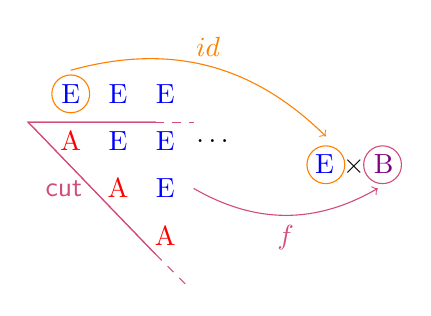
\begin{tikzpicture}[scale = 0.6]
    \foreach \y in {0,...,2}
    {\foreach \x in {\y,...,2}
      \draw (\x+1, -\y) node[color=blue]{E} ;
    }
    \foreach \x in {1,...,3} \draw (\x, -\x) node[color=red]{A} ;
    \draw(4,-1) node{$\ldots$};

     \draw (7,-1.5) node{{\color{blue} E} $\times$ {\color{violet} B}} ;
    \draw[color=orange] (1,0) circle(0.4cm);
    \draw[color=orange] (6.4,-1.5) circle(0.4cm);
    \draw[color=purple!70]  (2.8, -3.4) --
     (0.1,-0.6) -- (2.8,-0.6);
    \draw[color=purple!70, dashed]  (2.8,-0.6) -- (3.6,-0.6);
    \draw[color=purple!70, dashed]  (2.8,-3.4) -- (3.5,-4.1);

    \draw[color=purple!70] (7.6,-1.5) circle(0.4cm);

     \draw[->, color = orange] (1,0.5) to [bend left] node[auto,
     swap, above]{$id$} (6.4,-0.9) ; 
    \draw[->, color = purple!70] (3.6,-2) to [bend right] node[auto,
    swap, below]{$f$} (7.5,-2) ; 
    \draw[color=purple!70]  (2.8,-0.6) --  (0.1,-0.6) -- node[auto, swap,
    left]{$\cut$}(2.8, -3.4);
  \end{tikzpicture}
 \end{center}
\end{frame}

\begin{frame}
 \frametitle{A specified $\cut$ for any coalgebra}
  \begin{itemize}
    \item we were not able to define $\cut$ categorically
    \item fix: every coalgebra $(T,r)$ comes with a \fat{specified}
       \[ c_A : T (E\times A) \to TA \]
          and equations characterizing $c$
    \item $c^{\Tri} := \cut$ for $\Tri$ uniquely determined by these equations
   \end{itemize}
 \begin{lemma}[for real this time]
  $(\Tri,\cut,\tail)$ is terminal in the category of coalgebras $(T,c,r)$.
 \end{lemma}

\end{frame}

% TODO: conclusion / summary frame

\begin{comment}
\begin{frame}
 \frametitle{Closing remarks}
 
   \begin{block}{Higher order compatibility}
    Observing that $\Setoid$ is cartesian closed, one can encode
       \[ f \sim g  \Longrightarrow \redec~f \sim \redec~g\]
    in definition of coalgebra for signature of $\Tri$
   \end{block}
\end{frame}
\end{comment}
 
\begin{frame}
  \frametitle{Formalization}
   \begin{block}{Mechanization in the proof assistant \texttt{Coq}}
      \begin{itemize}\setlength{\itemsep}{1em}
       \item helped to find a mistake we made (already made by Abel, Matthes \& Uustalu '05)
       \item reuses code by Matthes \& Picard '11
       \item 3000 lines of code, among which 1500 by MP '11
       \item fully constructive and axiom-free
       \item tedious: coinduction in \texttt{Coq} cumbersome
      \end{itemize}
   \end{block}
   
\end{frame}

\begin{frame}
 \frametitle{Summary}
  
   \begin{itemize}\setlength{\itemsep}{1em}
    \item Coinductive type + bisimilarity as setoid in IMLTT
    \item $\stream$ and $\Tri$ are \fat{relative} comonads
%     \item Ad hoc notion of weak constructive comonad is instance of relative comonad
    \item Develop comodules over relative comonads
    \item Terminal algebra semantics for $\stream$ and $\Tri$
    \item Bisimilarity and redecoration are part of universal object
    \item $\Tri$ not as straightforward as the $\lambda$-calculus because of $\cut$
    \item Mechanization in \texttt{Coq}
   \end{itemize}

   \pause \begin{center} Thanks for your attention \end{center}
   
\end{frame}



\begin{frame}
 \frametitle{Some references}
 
  
  
  \begin{block}{Some references}
   \begin{itemize}
    \item Altenkirch, Chapman \& Uustalu: \emph{Monads need not be endofunctors}
    \item Hirschowitz \& Maggesi: \emph{Modules over Monads and Linearity}
    \item Matthes \& Picard: \emph{Verification of Redecoration for Infinite Triangular Matrices using Coinduction}
    \item preprint about this work on the arXiv
   \end{itemize}
  \end{block}

  TikZ pictures used with permission from Matthes and Picard
 
\end{frame}


\end{document}


% TODO: show cut operation
% TODO: reuse code

